Najniższy stopień automorfizmu przyjętego przez niezależny weryfikator: \textbf{6} (znane ograniczenie górne: $16$). Weryfikator sprawdza dokładnie, w arytmetyce liczb wymiernych, warunki $F(p_i)=q_i$, odwracalność (odwrotność wielomianowa o współczynnikach wymiernych) oraz stopień. Stopień ten jest ograniczeniem \emph{górnym}; o ograniczeniach dolnych mówią wyłącznie twierdzenia opisane w dalszych częściach raportu.

Przyjęte rozwiązania: 5; odrzucone: 0.
\begin{center}\small\begin{tabular}{rlp{5.2cm}p{5.6cm}}\toprule Stopień & Czynniki & Autor & Plik\\\midrule
6 & 2$\cdot$3 & iter02/zad3 & \texttt{praca/\allowbreak{}iter02/\allowbreak{}zad3/\allowbreak{}rozwiazanie\_st6\_ladne.json}\\
6 & 3$\cdot$2 & iter01/zad1 & \texttt{praca/\allowbreak{}iter01/\allowbreak{}zad1/\allowbreak{}rozwiazanie\_st6.json}\\
6 & 3$\cdot$2 & iter01/zad2 & \texttt{praca/\allowbreak{}iter01/\allowbreak{}zad2/\allowbreak{}rozwiazanie\_st6\_32.json}\\
6 & 2$\cdot$3 & iter01/zad2 & \texttt{praca/\allowbreak{}iter01/\allowbreak{}zad2/\allowbreak{}rozwiazanie\_st6\_23.json}\\
16 & 4$\cdot$4 & konstrukcja bazowa (skrypt przygotowany przed eksperymentem) & \texttt{praca/\allowbreak{}iter00/\allowbreak{}baza/\allowbreak{}rozwiazanie\_bazowe.json}\\
\bottomrule\end{tabular}\end{center}
\subsection*{Najlepsze znalezione odwzorowanie}
A\ensuremath{\circ}(x+g(y),y)\ensuremath{\circ}(x,y+f(x))\ensuremath{\circ}B, multistopien (2,3), najczytelniejsze z przeszukania kierunkow |.|<=3
\noindent $F = \varphi_n\circ\dots\circ\varphi_1$, gdzie (w kolejności działania):
\begin{align*}
\varphi_{1}&\colon (x,y)\mapsto\left(y,\ - 3 x + y - \frac{8}{3}\right)\\\varphi_{2}&\colon (x,y)\mapsto\left(x,\ y + \left(\frac{8 x^{2}}{3}\right)\right)\\\varphi_{3}&\colon (x,y)\mapsto\left(x + \left(- \frac{5 y^{3}}{96} - \frac{y^{2}}{24}\right),\ y\right)\\\varphi_{4}&\colon (x,y)\mapsto\left(- x - \frac{5 y}{24} - \frac{1}{6},\ - 3 x - \frac{13 y}{8} - \frac{1}{2}\right)
\end{align*}
Postać rozwinięta:
\begin{flushleft}\small
$F_1(x,y) = - \frac{45 x^{3}}{32} + \frac{15 x^{2} y^{2}}{4} + \frac{45 x^{2} y}{32} - \frac{27 x^{2}}{8} - \frac{10 x y^{4}}{3} - \frac{5 x y^{3}}{2} + \frac{177 x y^{2}}{32} + \frac{9 x y}{4} - \frac{49 x}{24} + \frac{80 y^{6}}{81} + \frac{10 y^{5}}{9} - \frac{9 y^{4}}{4} - \frac{187 y^{3}}{96} + \frac{311 y^{2}}{216} - \frac{23 y}{72} - \frac{49}{162}$\par\medskip
$F_2(x,y) = - \frac{135 x^{3}}{32} + \frac{45 x^{2} y^{2}}{4} + \frac{135 x^{2} y}{32} - \frac{81 x^{2}}{8} - 10 x y^{4} - \frac{15 x y^{3}}{2} + \frac{531 x y^{2}}{32} + \frac{27 x y}{4} - \frac{25 x}{8} + \frac{80 y^{6}}{27} + \frac{10 y^{5}}{3} - \frac{27 y^{4}}{4} - \frac{187 y^{3}}{32} + \frac{119 y^{2}}{72} - \frac{47 y}{24} + \frac{95}{54}$
\end{flushleft}
\IfFileExists{gen/najlepsze.pdf}{\begin{figure}[h!]\centering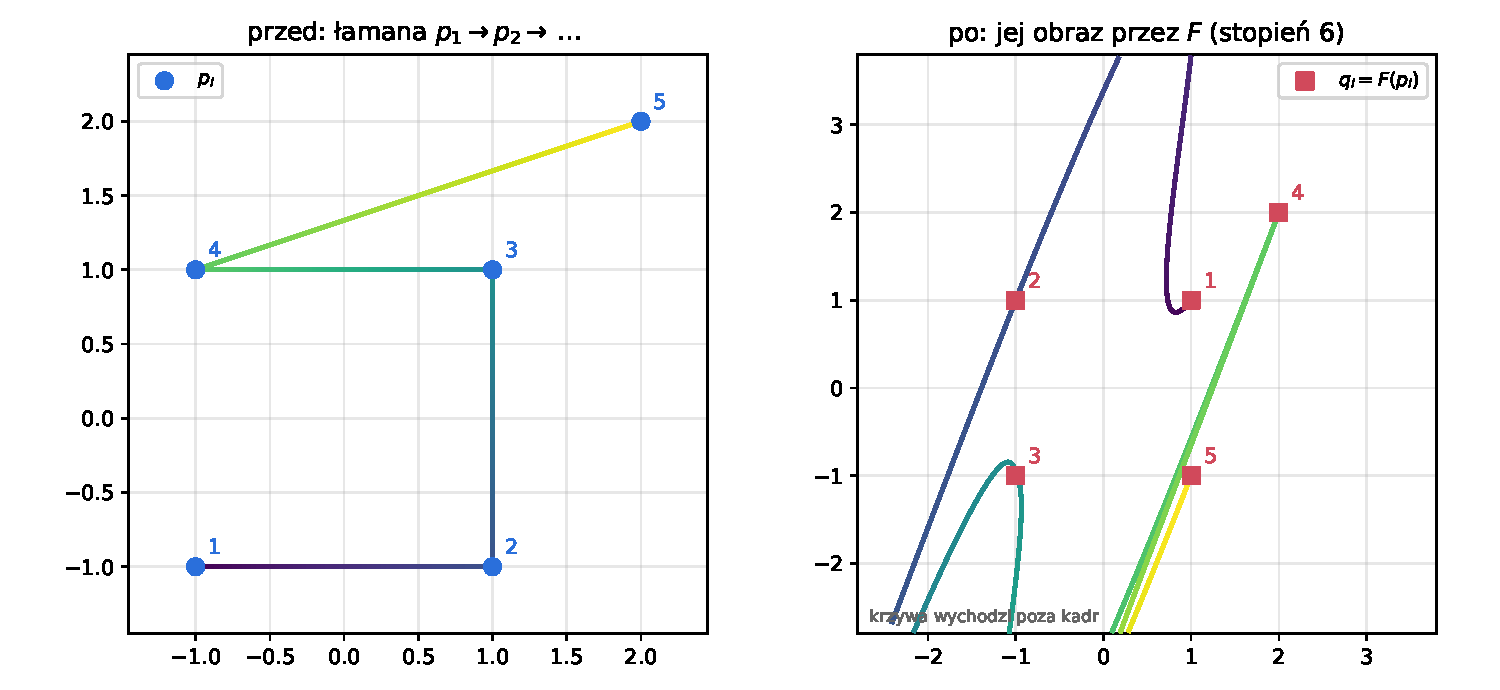
\includegraphics[width=\textwidth]{gen/najlepsze.pdf}\caption{Łamana $p_1\to\dots\to p_m$ (lewa) i jej obraz przez najlepsze znalezione $F$ (prawa); barwa wskazuje położenie wzdłuż łamanej.}\end{figure}}{}
\IfFileExists{gen/czynniki.pdf}{\begin{figure}[h!]\centering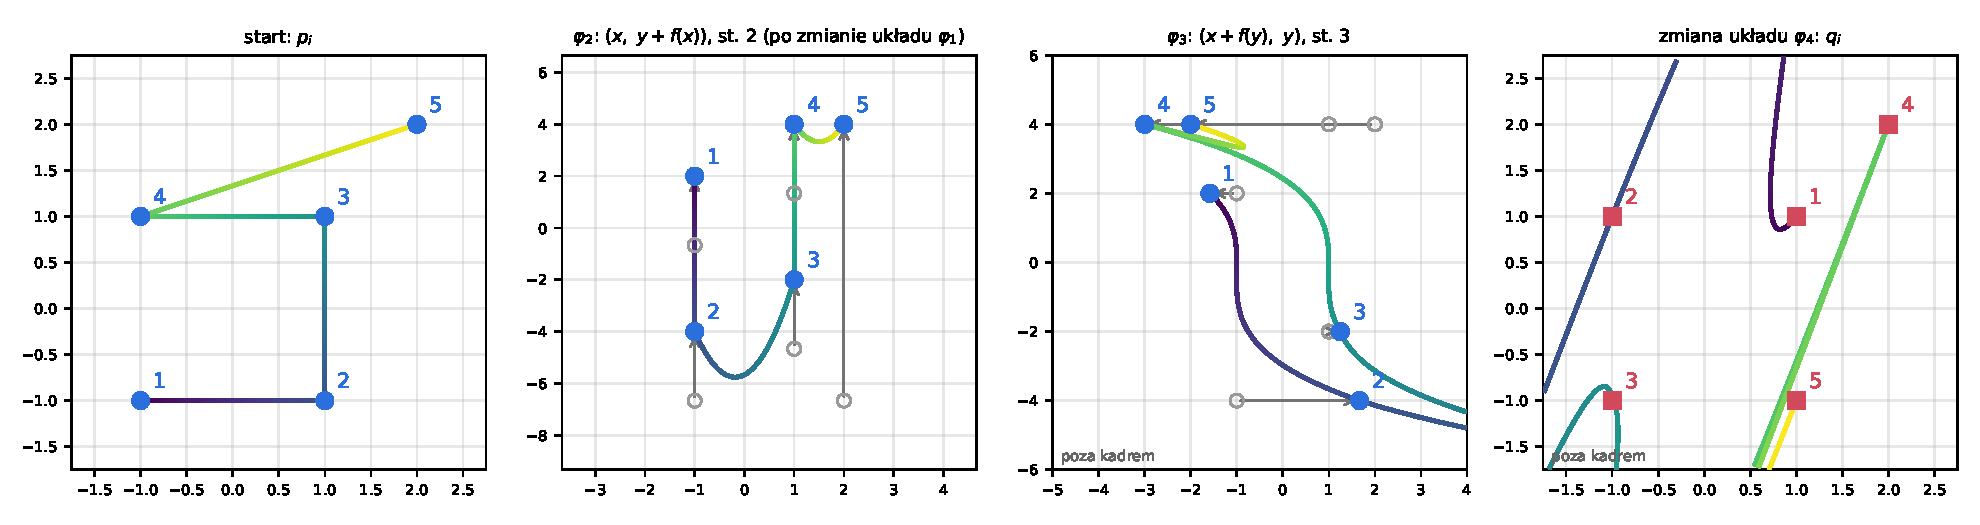
\includegraphics[width=\textwidth]{gen/czynniki.pdf}\caption{Działanie kolejnych czynników $\varphi_k$ najlepszego $F$ na punkty i łamaną. Czynnik trójkątny przesuwa punkty tylko pionowo albo tylko poziomo; każdy panel ma własny kadr.}\end{figure}}{}
\IfFileExists{gen/postep.pdf}{\begin{figure}[h!]\centering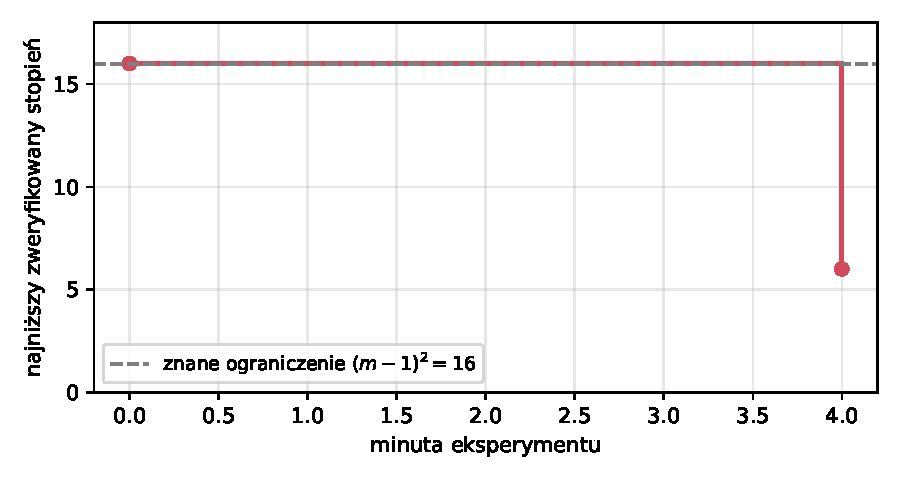
\includegraphics[width=0.7\textwidth]{gen/postep.pdf}\caption{Najniższy zweryfikowany stopień w kolejnych minutach eksperymentu.}\end{figure}}{}
